\question \textbf{Linear progressive alignment}

Construct an MSA from seq1, seq2, seq3 and a phylogenetic tree by using the progressive alignment method specified below.

\begin{figure}[H]
      \centering
      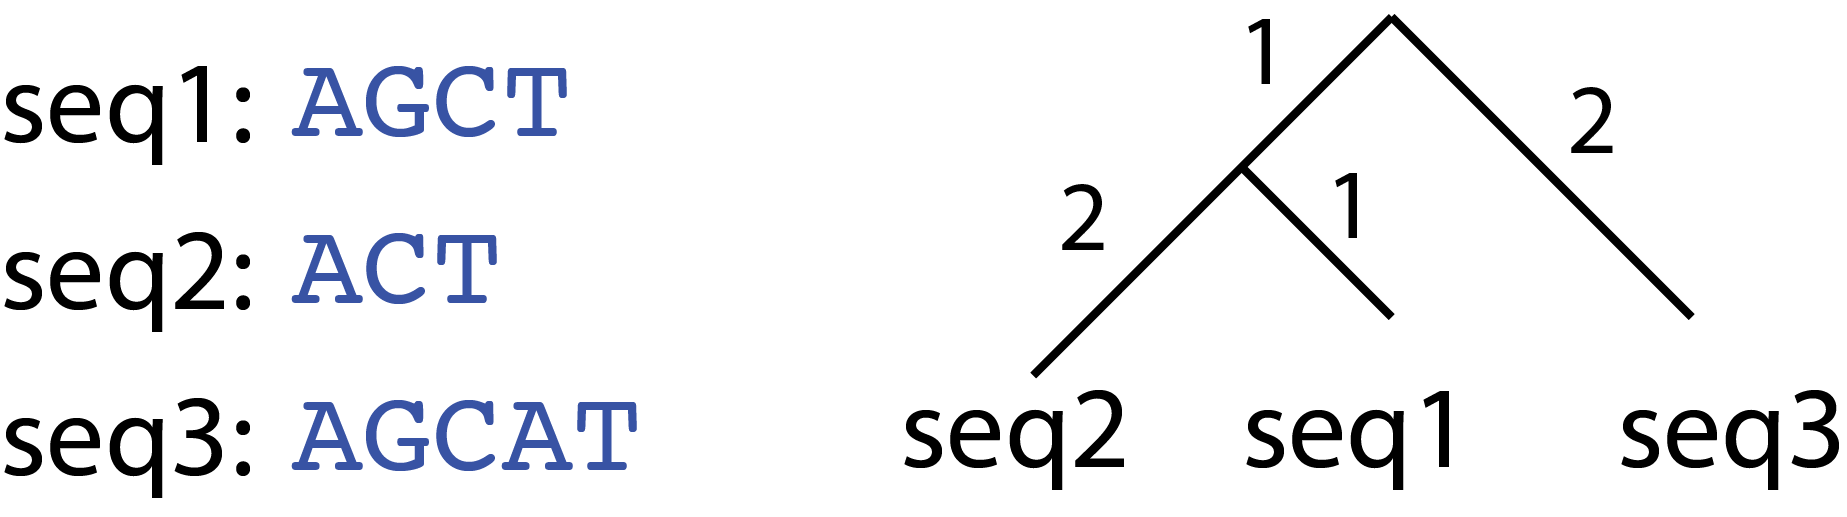
\includegraphics[width=0.4 \textwidth]{fig10/progressive_alignment_tree.png}
\end{figure}

\begin{itemize}
\item Clustering: Linear clustering
\item Aligning method: Pair-guided alignment
\item Aligning order: Use the specified tree 
\item Pairwise DP: Global alignment with linear gap penalty
\item DP scoring scheme: match (10), mismatch (-5), gap penalty (10)
\end{itemize}

\begin{parts}

\vspace{0.1 in}

%% (a)
  \part What is the aligning order that can be defined by the given tree? 

\begin{solution}[0.7 in]
\begin{verbatim}
1: Seq2 & Seq1
2: Seq1 & Seq3
\end{verbatim}
\end{solution}

%% (b)
  \part Solve the first pairwise alignment.

\begin{solution}[0.7 in]
\begin{verbatim}
Seq2: A-CT
Seq1: AGCT
\end{verbatim}
\end{solution}

%% (c)
  \part Solve the second pairwise alignment.

\begin{solution}[0.7 in]
\begin{verbatim}
Seq1: AGC-T
Seq3: AGCAT
\end{verbatim}
\end{solution}

%% (d)
  \part Find the optimal MSA by combining the first and the second alignments.

\begin{solution}[1.1 in]
\begin{verbatim}
Seq1: AGC-T
Seq2: A-C-T
Seq3: AGCAT
\end{verbatim}
\end{solution}

%% (e)
  \part What is the SP score of the optimal MSA?

\begin{solution}[1.7 in]
\begin{verbatim}
Seq1 & Seq2: 20
Seq1 & Seq3: 30
Seq2 & Seq3: 10

SP: 60
\end{verbatim}
\end{solution}

\end{parts}
